\documentclass[border=1pt]{standalone}
%\usetikzlibrary{...}% tikz package already loaded by 'tikz' option
\usepackage{tikz}
\usetikzlibrary{matrix, fit}
\usetikzlibrary{backgrounds}
\begin{document}
\thispagestyle{empty}
$
\hspace{-10pt}
\vcenter{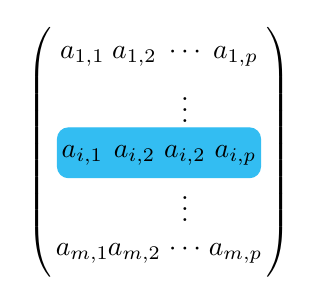
\begin{tikzpicture}
\matrix [matrix of math nodes,
         nodes={rectangle, 
                minimum size=1.8em, text depth=0.25ex,
                inner sep=0pt, outer sep=0pt,
                anchor=center},
         column sep=-0.5\pgflinewidth,
         row sep=-0.5\pgflinewidth,
         inner sep=0pt,
         left delimiter=(, right delimiter=),
         row 2 column 2/.append style={nodes={draw=cyan,fill=cyan}},
         ] (m)
{
a_{1,1} & & a_{1,2}  & & \cdots & & a_{1,p} \\
 & &   & & \vdots   & & \\
a_{i,1}& & a_{i,2}& & a_{i,2} & &  a_{i,p}  \\
 & &   & & \vdots   && \\
a_{m,1}& & a_{m,2}& & \cdots & &  a_{m,p}  \\
};
\begin{scope}[on background layer]
    \filldraw[cyan!80, rounded corners] (m-3-1.north west) -- 
        (m-3-1.south west) -- (m-3-7.south east)-- (m-3-7.north east)-- 
        cycle;
\end{scope} 
\end{tikzpicture}
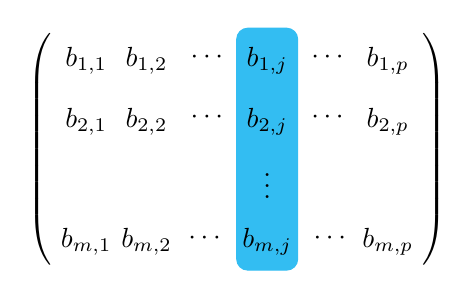
\begin{tikzpicture}
\matrix [matrix of math nodes,
         nodes={rectangle, 
                minimum size=2.2em, text depth=0.25ex,
                inner sep=0pt, outer sep=0pt,
                anchor=center},
         column sep=-0.5\pgflinewidth,
         row sep=-0.5\pgflinewidth,
         inner sep=0pt,
         left delimiter=(, right delimiter=),
         ] (m)
{
b_{1,1} &  b_{1,2} &  \cdots &  b_{1,j} &  \cdots &  b_{1,p} \\
b_{2,1} &  b_{2,2} &  \cdots &  b_{2,j} &  \cdots &  b_{2,p} \\
  &    &   &  \vdots  &   &  \\
b_{m,1} &  b_{m,2} &  \cdots\, &  b_{m,j} &  \,\cdots &  b_{m,p} \\
};
\begin{scope}[on background layer]
    \filldraw[cyan!80, rounded corners] (m-1-4.north west) -- 
        (m-1-4.north east) -- (m-4-4.south east)-- (m-4-4.south west)-- 
        cycle;
\end{scope} 
\end{tikzpicture}}\hspace{-80pt}=\hspace{-15pt}
\vcenter{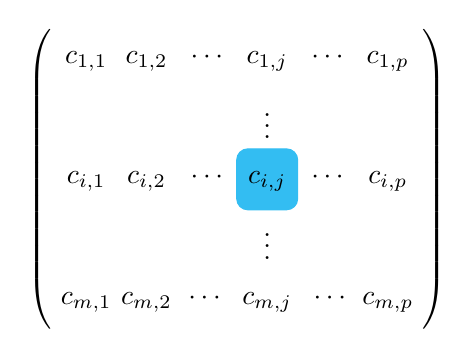
\begin{tikzpicture}
\matrix [matrix of math nodes,
         nodes={rectangle, 
                minimum size=2.2em, text depth=0.25ex,
                inner sep=0pt, outer sep=0pt,
                anchor=center},
         column sep=-0.5\pgflinewidth,
         row sep=-0.5\pgflinewidth,
         inner sep=0pt,
         left delimiter=(, right delimiter=),
         ] (m)
{
c_{1,1} &  c_{1,2} &  \cdots &  c_{1,j} &  \cdots &  c_{1,p} \\
 &   &   &  \vdots &   &   \\
 c_{i,1} &  c_{i,2} &  \cdots &  c_{i,j} &  \cdots &  c_{i,p} \\
  &    &   &  \vdots  &   &  \\
c_{m,1} &  c_{m,2} &  \cdots\, &  c_{m,j} &  \,\cdots &  c_{m,p} \\
};
\begin{scope}[on background layer]
    \filldraw[cyan!80, rounded corners] (m-3-4.north west) -- 
        (m-3-4.north east) -- (m-3-4.south east)-- (m-3-4.south west)-- 
        cycle;
\end{scope} 
\end{tikzpicture}}\hspace{-170pt}
$
\end{document}